\documentclass[a5paper, 10pt]{tekst}

\usepackage{titlesec}
\usepackage{indentfirst}

\begin{document}
	\thispagestyle{empty}
	\onehalfspacing
	\titleformat*{\section}{\sffamily\bfseries}
	\sffamily
	
	\begin{center}
		\Huge \p{\f{壁}{かべ}の}\p{\f{穴}{あな}}、\p{\f{第}{だい}}\p{\f{三}{さん}\f{話}{わ}}
	\end{center}
	
	\begin{figure}[h]
		\centering
		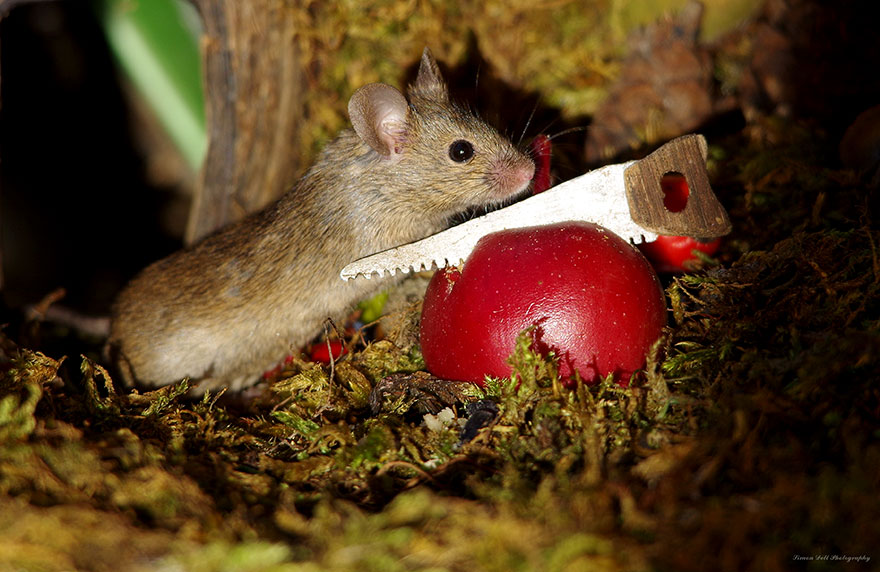
\includegraphics[width=0.5\linewidth]{figures/ねずみ4.jpeg}
	\end{figure}
	
	{\Large\sloppy
		\noindent\ruby{僕}{ぼく}は、 \ruby{壁}{かべ}の \ruby{穴}{あな}から そっと \ruby{外}{そと}に \ruby{出}{で}た。 \ruby{壁}{かべ}の \ruby{穴}{あな}は、 \ruby{仏壇}{ぶつだん}の \ruby{後}{うし}ろに ある。 きっと、 \ruby{人間}{にんげん}\ruby{達}{たち}は、 この \ruby{穴}{あな}を \ruby{隠}{かく}す ために、 \ruby{仏壇}{ぶつだん}を ここに \ruby{置}{お}いたん だろう。 \ruby{前}{まえ}に \ruby{住}{す}んでいた \ruby{家}{いえ}も そう だった。 そこは、 \ruby{壁}{かべ}の \ruby{穴}{あな}の\ruby{前}{まえ}に、 \ruby{本棚}{ほんだな}が \ruby{置}{お}いて あった。 \ruby{僕}{ぼく}\ruby{達}{たち} にとって、 \ruby{隠}{かく}された \ruby{壁}{かべ}の \ruby{穴}{あな}の \ruby{中}{なか}は、 \ruby{完璧}{かんぺき}な \ruby{家}{いえ} だった。 
		
		\noindent \ruby{僕}{ぼく}は、 \ruby{仏壇}{ぶつだん}と \ruby{壁}{かべ}の \ruby{間}{あいだ}に ある \ruby{隙間}{すきま}の \ruby{道}{みち}を \ruby{通}{とお}って、 \ruby{廊下}{ろうか}の \ruby{方}{ほう}へと \ruby{向}{む}かった。 \ruby{廊下}{ろうか}を \ruby{照}{て}らす \ruby{朝日}{あさひ}が \ruby{眩}{まぶ}しかった。 \ruby{今日}{きょう}も また、 \ruby{暑}{あつ}く なりそう だなぁと \ruby{思}{おも}った。
		
		\noindent \ruby{遠}{とお}くから、「 クミコ、 \ruby{朝}{あさ}ごはんよ~」 と、 クミコの \ruby{母}{かあ}ちゃんの \ruby{声}{こえ}が \ruby{聞}{き}こえた。 \ruby{僕}{ぼく}は、 そっと \ruby{仏壇}{ぶつだん}の \ruby{陰}{かげ}から クミコを \ruby{探}{さが}した。 クミコは、 \ruby{廊下}{ろうか}に \ruby{寝}{ね}っ\ruby{転}{ころ}がっていた。 \ruby{座布団}{ざぶとん}の \ruby{上}{うえ}で、 \ruby{日向}{ひなた}ぼっこを している ように \ruby{見}{み}えた。 \ruby{座布団}{ざぶとん}から、 クミコの \ruby{足}{あし}が はみ\ruby{出}{だ}していた。 あったかくて \ruby{気持}{きも}ち よさそうな \ruby{場所}{ばしょ} だった。 
		
	}\clearpage
	\titleformat*{\section}{\rmfamily\bfseries}
	\rmfamily
	
	\section*{Vokabular}
	\begin{multicols}{2}[\centering\textbf{Bitno}]\noindent
		\dictentry{隠す}{かくす}{\item skrivati}{glagol (五)}
		\dictentry{本棚}{ほんだな}{\item polica za knjige}{imenica}
		\dictentry{完璧}{かんぺき}{\item savršen}{na-pridjev}
		\dictentry{隙間}{すきま}{\item pukotina}{imenica}
		\dictentry{眩しい}{まぶしい}{\item sjajan, zračeći(zasljepljujuć?)}{i-pridjev}
		\dictentry{遠く}{とおく}{\item daleko}{imenica, prilog, no-pridjev}
		\dictentry{寝っ転がる}{ねっころがる}{\item zaleći}{glagol (五)}
		\dictentry{日向ぼっこ}{ひなたぼっこ}{\item izležavanje na suncu}{imenica, suru-glagol}
		\dictentry{はみ出す}{はみだす}{\item proviriti(stršati?)}{glagol (五)}
	\end{multicols}
	
	\begin{multicols}{2}[\centering\textbf{Ostalo}]
		\dictentry{僕}{ぼく}{\item ja, muški}{zamjenica}
		\dictentry{壁}{かべ}{\item zid}{imenica}
		\dictentry{穴}{あな}{\item rupa}{imenica}
		\dictentry{外}{そと}{\item vani}{imenica}
		\dictentry{出る}{でる}{\item izaći}{glagol (一)}
		\dictentry{仏壇}{ぶつだん}{\item Budistički oltar (kućni)}{imenica}
		\dictentry{後ろ}{うしろ}{\item iza, otraga}{imenica, no-pridjev}
		\dictentry{人間}{にんげん}{\item čovjek}{imenica}
		\dictentry{達}{たち}{\item plural}{sufiks}
		\dictentry{置く}{おく}{\item smjestiti(staviti?)}{glagol (五)}
		\dictentry{前}{まえ}{\item prije}{priložna imenica}
		\dictentry{住む}{すむ}{\item stanovati}{glagol (五)}
		\dictentry{家}{いえ}{\item kuća}{imenica}
		\dictentry{中}{なか}{\item unutra}{imenica, no-pridjev}
		\dictentry{間}{あいだ}{\item prostor (između)}{imenica}
		\dictentry{道}{みち}{\item put}{imenica}
		\dictentry{通る}{とおる}{\item prolaziti pored}{glagol (五)}
		\dictentry{廊下}{ろうか}{\item hodnik}{imenica}
		\dictentry{方}{ほう}{\item smjer, način}{imenica}
		\dictentry{向かう}{むかう}{\item ići prema(uputiti se prema?)}{glagol (五)}
		\dictentry{照らす}{てらす}{\item obasjavati}{glagol (五)}
		\dictentry{朝日}{あさひ}{\item jutarnje sunce}{imenica}
		\dictentry{今日}{きょう}{\item danas}{imenica}
		\dictentry{暑い}{あつい}{\item topao}{i-pridjev}
		\dictentry{思う}{おもう}{\item misliti}{glagol (五)}
		\dictentry{朝ごはん}{あさごはん}{\item doručak}{imenica}
		\dictentry{母ちゃん}{かあちゃん}{\item mama}{imenica}
		\dictentry{声}{こえ}{\item glas}{imenica}
		\dictentry{聞こえる}{きこえる}{\item biti čut(čuti se?)}{glagol (五)}
		\dictentry{探す}{さがす}{\item tražiti}{glagol (五) }
		\dictentry{座布団}{ざぶとん}{\item zabuton (jastuk)}{imenica}
		\dictentry{上}{うえ}{\item iznad}{imenica, no-pridjev, prilog}
		\dictentry{見える}{みえる}{\item biti viđen(vidjeti se?)}{glagol (五)}
		\dictentry{足}{あし}{\item noga}{imenica}
		\dictentry{気持ち}{きもち}{\item osjećaj}{imenica}
		\dictentry{場所}{ばしょ}{\item mjesto}{imenica}
	\end{multicols}
	
	\clearpage
	
	\section*{Domaća zadaća}
	\begin{enumerate}
		\item Napišite kratku priču ili par rečenica koristeći riječi iz kutije ispod.
		Rečenice ili tekst ne moraju nužno biti vezane uz sam tekst.
		\begin{center}
			\vspace{0.5em}
			\fbox{隠す ・ 本棚 ・ 寝っ転がる ・ 日向ぼっこ}\vspace{1.4em}
			\rule{\linewidth}{0.5pt}\\[0.6em]
			\rule{\linewidth}{0.5pt}\\[0.6em]
			\rule{\linewidth}{0.5pt}\\[0.6em]
			\rule{\linewidth}{0.5pt}\\[0.6em]
			\rule{\linewidth}{0.5pt}\\[0.6em]
			\rule{\linewidth}{0.5pt}\\[0.6em]
			\rule{\linewidth}{0.5pt}
		\end{center}
		
		\item Odgovorite na pitanja:
		\begin{enumerate}[label=(\roman*)]
			\raggedright
			\item\vspace{0.5em}\p{\f{壁}{かべ}の}\p{\f{穴}{あな}は}\p{どこに}\p{ある?}
			\rule{\linewidth}{0.5pt}\\[0.6em]
			\rule{\linewidth}{0.5pt}
			\item\vspace{0.5em}\p{\f{語}{かた}り}\p{\f{手}{て}は、}\p{なぜ}\p{\f{人間}{にんげん}たちは}\p{\f{仏壇}{ぶつだん}や}\p{\f{本棚}{ほんだな}を}\p{\f{壁}{かべ}の}\p{\f{穴}{あな}の}\p{前に}\p{\f{置}{お}くの、だと}\p{\f{思}{おも}って}\p{いる?}
			\rule{\linewidth}{0.5pt}\\[0.6em]
			\rule{\linewidth}{0.5pt}
			\item\vspace{0.5em}\p{\f{廊下}{ろうか}に}\p{出る}\p{ために}\p{何を}\p{する}\p{\f{必要}{ひつよう}が}\p{ある?}
			\rule{\linewidth}{0.5pt}\\[0.6em]
			\rule{\linewidth}{0.5pt}
			\item\vspace{0.5em}\p{クミコの}\p{お}\p{\f{母}{おかあ}さんは}\p{\f{何}{なん}の}\p{ために}\p{クミコを}\p{\f{呼}{よ}んで}\p{いる?}
			\rule{\linewidth}{0.5pt}\\[0.6em]
			\rule{\linewidth}{0.5pt}
			\item\vspace{0.5em}\p{クミコは}\p{\f{何}{なん}の}\p{上に}\p{いた?}
			\rule{\linewidth}{0.5pt}\\[0.6em]
			\rule{\linewidth}{0.5pt}
		\end{enumerate}		
		\item Nadopunite sljedeće rečenice riječima iz kutije ispod:
		\begin{center}
			\choicebox{眩しい ・ 隙間 ・ 隠している ・ 寝っ転がっている ・ 本棚\\完璧 ・ 遠く ・ はみ出している ・ 日向ぼっこ }
		\end{center}
		\begin{enumerate}[label=(\roman*)]
			\raggedright
			
			\vspace{0.5em}\item \p{サダコは}\p{\f{顔}{かお}を}\p{\f{髪}{かみ}で\ansline{}から}\p{よく}\p{\f{見}{み}えない。}
			\item \p{\f{私}{わたし}の\ansline{}は}\p{でかくて}\p{\f{古}{ふる}い、だから}\p{そこで}\p{\f{色}{いろ}んな}\p{\f{本}{ほん}が}\p{\f{見}{み}つけられるよ。}
			\item \p{\ansline{}な}\p{ワン}\p{ピースを}\p{\f{昨日}{きのう}\f{店}{てん}に}\p{\f{見}{み}つけたけど}\p{\f{今月}{こんげつ}\f{金}{かね}は}\p{ちょっと}\p{きついので}\p{\f{買}{か}わなかった。}
			\item \p{\f{雨}{あめ}が}\p{\f{屋根}{やね}の\ansline{}から}\p{ぽたぽた}\p{\f{落}{お}ちて}\p{いた。}
			\item \p{クエーサーとは、}\p{\f{非常}{ひじょう}に}\p{\f{遠方}{えんぽう}に}\p{ある、\ansline{}}\p{\f{輝}{かがや}きを}\p{\f{放}{はな}つ}\p{\f{天体}{てんたい}だ。}
			\item \p{\f{彼}{かれ}らは}\p{あまり\ansline{}に}\p{\f{行}{い}かない}\p{うちに}\p{\f{1人}{ひとり}の}\p{\f{老人}{ろうじん}に}\p{\f{会}{あ}った。}
			\item \p{\f{猫}{ねこ}\f{達}{たち}は}\p{こたつの}\p{\f{下}{した}で\ansline{}。}
			\item \p{\f{桜子}{さくらこ}さんは\ansline{}が}\p{\f{大好}{だいす}きなんだ、}\p{\f{特}{とく}に}\p{\f{自分}{じぶん}の}\p{\f{庭}{にわ}で}\p{ミカンの}\p{\f{木}{き}の}\p{\f{隣}{となり}で。}
			\item \p{「\f{母}{かあ}さん、}\p{\f{母}{かあ}さん、}\p{\f{枝}{えだ}は}\p{\f{土}{つち}から\ansline{}、}\p{\f{変}{へん}だよね。」と}\p{\f{幼}{おさな}い}\p{\f{武}{たけし}\f{君}{くん}が}\p{\f{大声}{おおごえ}で}\p{\f{自分}{じぶん}の}\p{お}\p{\f{母}{かあ}さんに}\p{\f{言}{い}った。}
		\end{enumerate}
	\end{enumerate}
\end{document}